\chapter{Практическая часть}

На рисунках~\ref{ex:uniform_1}--\ref{ex:uniform_2} представлены построенные графики по заданным параметрам для равномерного распределения.

\begin{figure}[ht!]
	\centering
	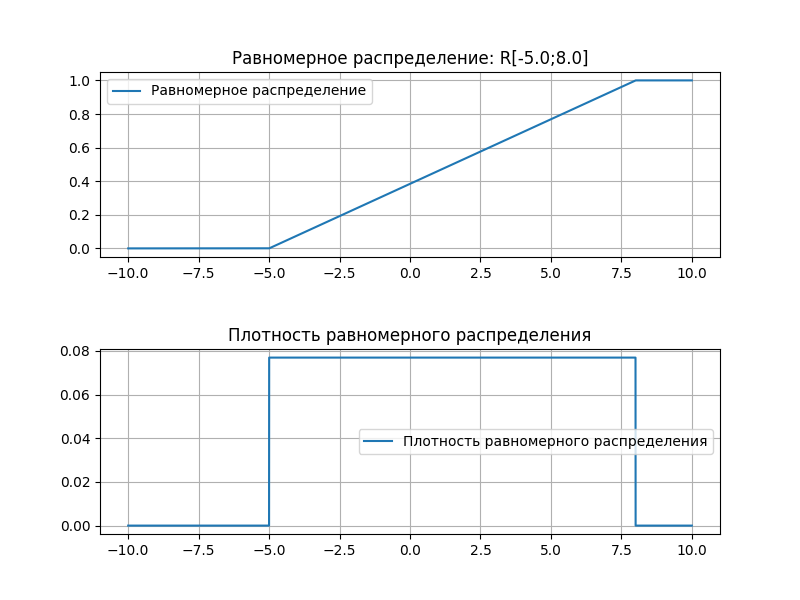
\includegraphics[width=1.0\linewidth]{img/uniform1.png}
	\caption{Равномерное распределение при a = -5 и b = 8}
	\label{ex:uniform_1}
\end{figure}

\clearpage

\begin{figure}[ht!]
	\centering
	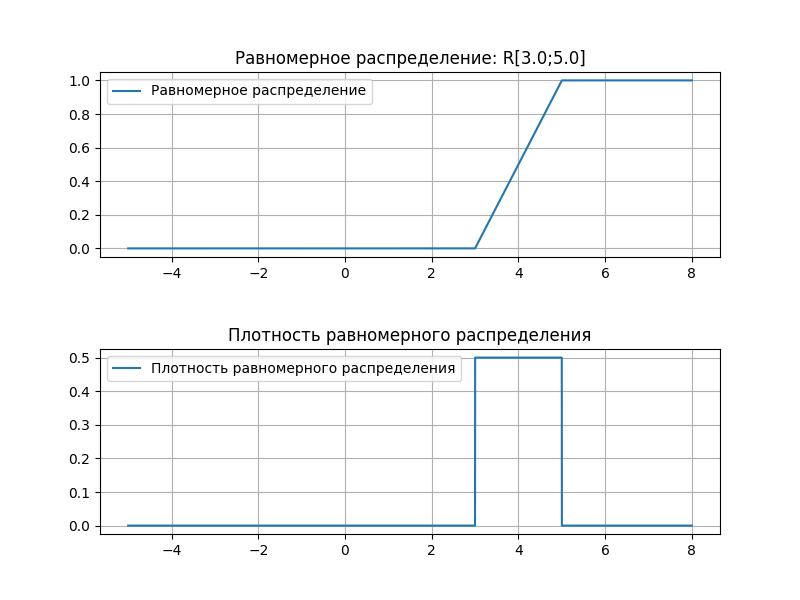
\includegraphics[width=1.0\linewidth]{img/uniform2.png}
	\caption{Равномерное распределение при a = 3 и b = 5}
	\label{ex:uniform_2}
\end{figure}

\clearpage

На рисунках~\ref{ex:n1}--\ref{ex:n3} представлены построенные графики по заданным параметрам для пуассоновского распределения.

\begin{figure}[ht!]
	\centering
	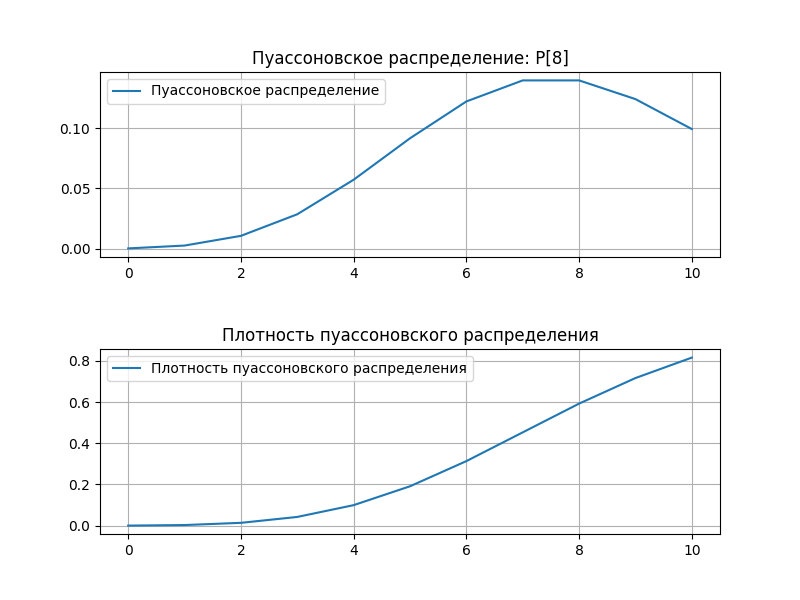
\includegraphics[width=1.0\linewidth]{img/poisson1.png}
	\caption{Пуассоновское распределение при $\lambda$ = 8}
	\label{ex:n1}
\end{figure}

\clearpage

\begin{figure}[ht!]
	\centering
	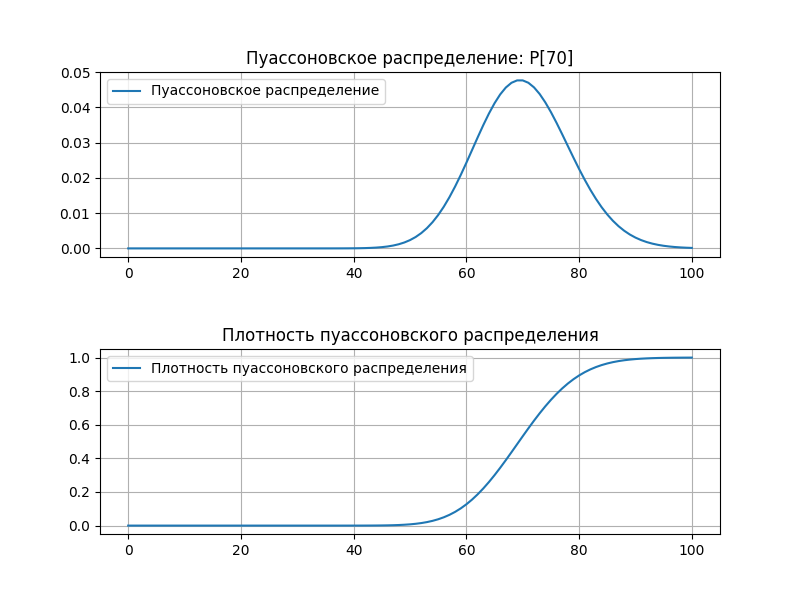
\includegraphics[width=1.0\linewidth]{img/poisson2.png}
	\caption{Пуассоновское распределение при $\lambda$ = 70}
	\label{ex:n2}
\end{figure}

\clearpage

\begin{figure}[ht!]
	\centering
	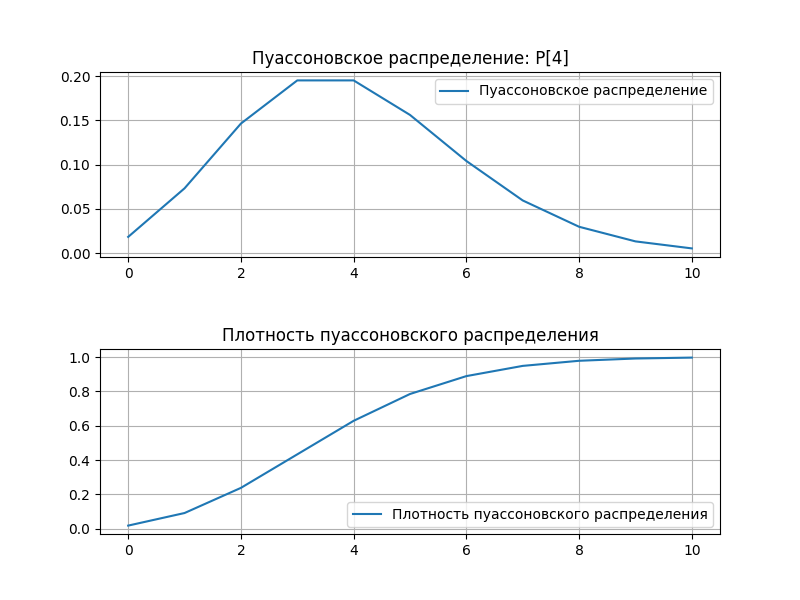
\includegraphics[width=1.0\linewidth]{img/poisson3.png}
	\caption{Пуассоновское распределение при $\lambda$ = 4}
	\label{ex:n3}
\end{figure}